\subsubsection{Guidance method's questionnaire.}
\label{subsubsec:results_questionnaires}

The data from the questionnaire for evaluating the user experience with each guidance method is also analysed. The higher the score, the more satisfied the user is with the method. It is essential to observe that this analysis does not include the base method as the questions are specific about each method and the base may vary among the participants. Also, there is no distinction between first and return rounds. Each questionnaire is answered only once for each method.

Table \ref{tab:questionnaire_average_blind} presents the score attributed to each method by each participant. The mean values are plotted in Figure \ref{fig:barplot_questionnaire_scene_blind} and show a dissatisfaction with the methods that only use vibration for communicating with the participant, i.e., the haptic belt and the virtual cane. 


\begin{table}[!htb]
\centering
\caption{ Guidance method questionnaire score felled by the blinded participants.}
\label{tab:questionnaire_average_blind}
\begin{tabular}{llrrrrr}
\toprule
{} &  Audio &  \begin{tabular}[c]{@{}l@{}}Haptic\\ Belt\end{tabular} &  \begin{tabular}[c]{@{}l@{}}Virtual\\ Cane\end{tabular} &  Mixture \\
Participant &        &                                                        &                                                         &          \\
\midrule
001C        &  0.774 &                                                  0.543 &                                                   0.629 &    0.865 \\
002C        &  0.857 &                                                  0.743 &                                                   0.543 &    0.935 \\
003C        &  0.929 &                                                  0.571 &                                                   0.543 &    0.745 \\
004C        &  0.881 &                                                  0.486 &                                                   0.400 &    0.730 \\
\bottomrule
\end{tabular}
\end{table}



\begin{figure}[!htb]
    \centering
    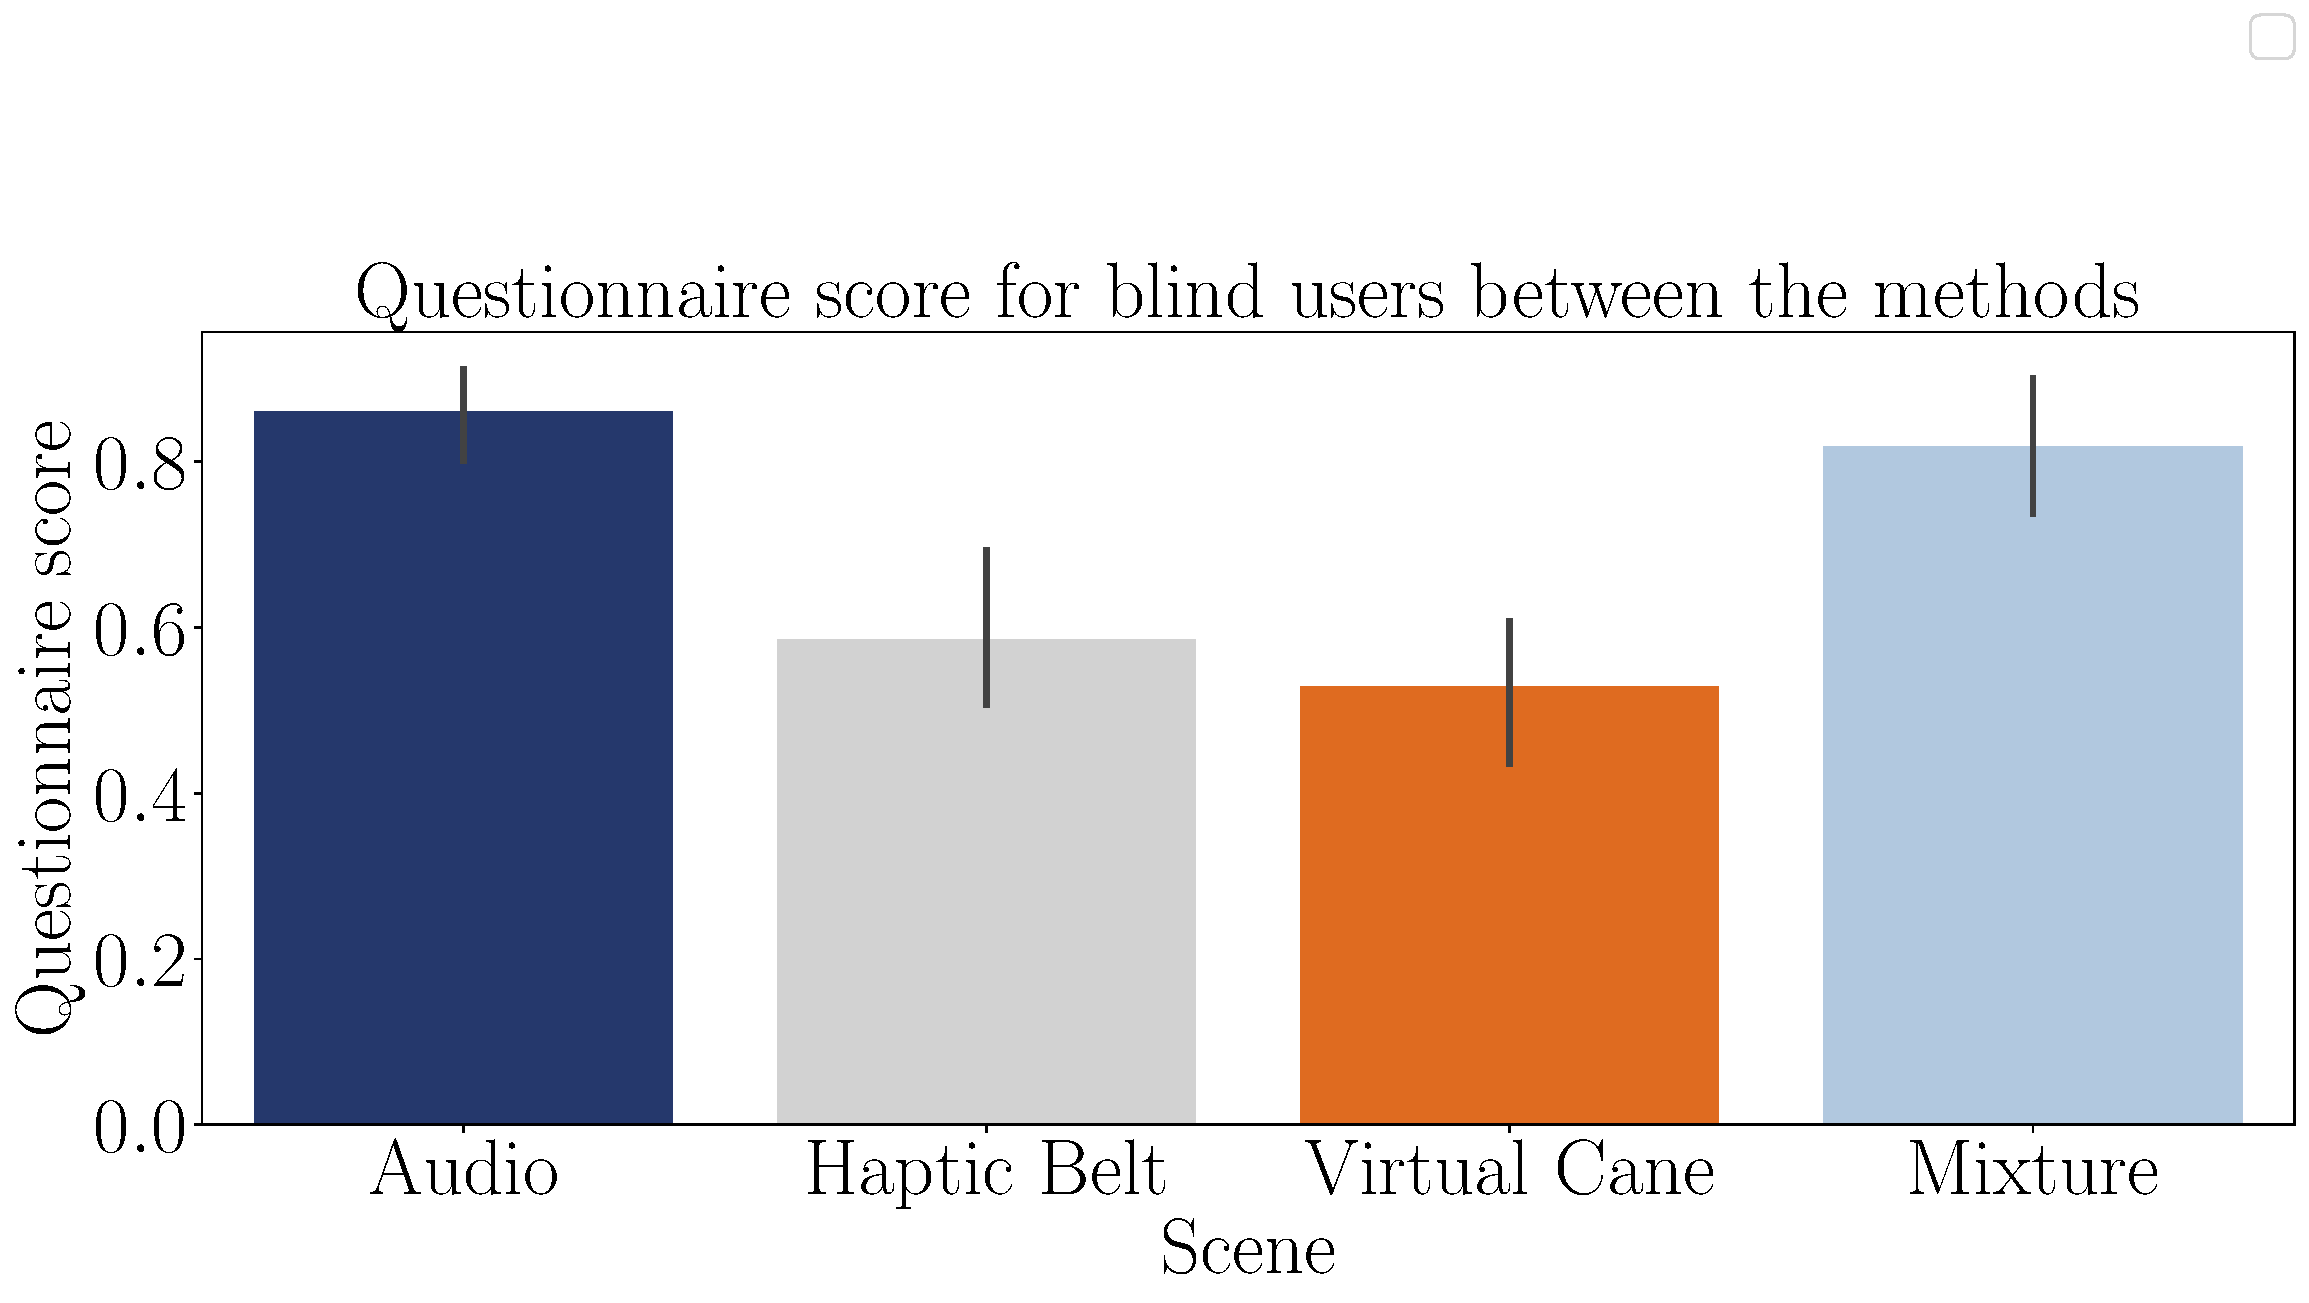
\includegraphics[width = \textwidth]{Resultados/Questionario/Figuras/pdf/barplot_questionnaire_scene_blind.pdf}
    \caption{Barplot of the average questionaire score of the blind participants on each method.}
    \label{fig:barplot_questionnaire_scene_blind}
\end{figure}

Figure \ref{fig:boxplot_quest_blind_scene} brings the questionnaire boxplot, which clearly shows the difference between two groups: haptic belt and virtual cane, and audio and mixture. 

\begin{figure}[!htb]
    \centering
    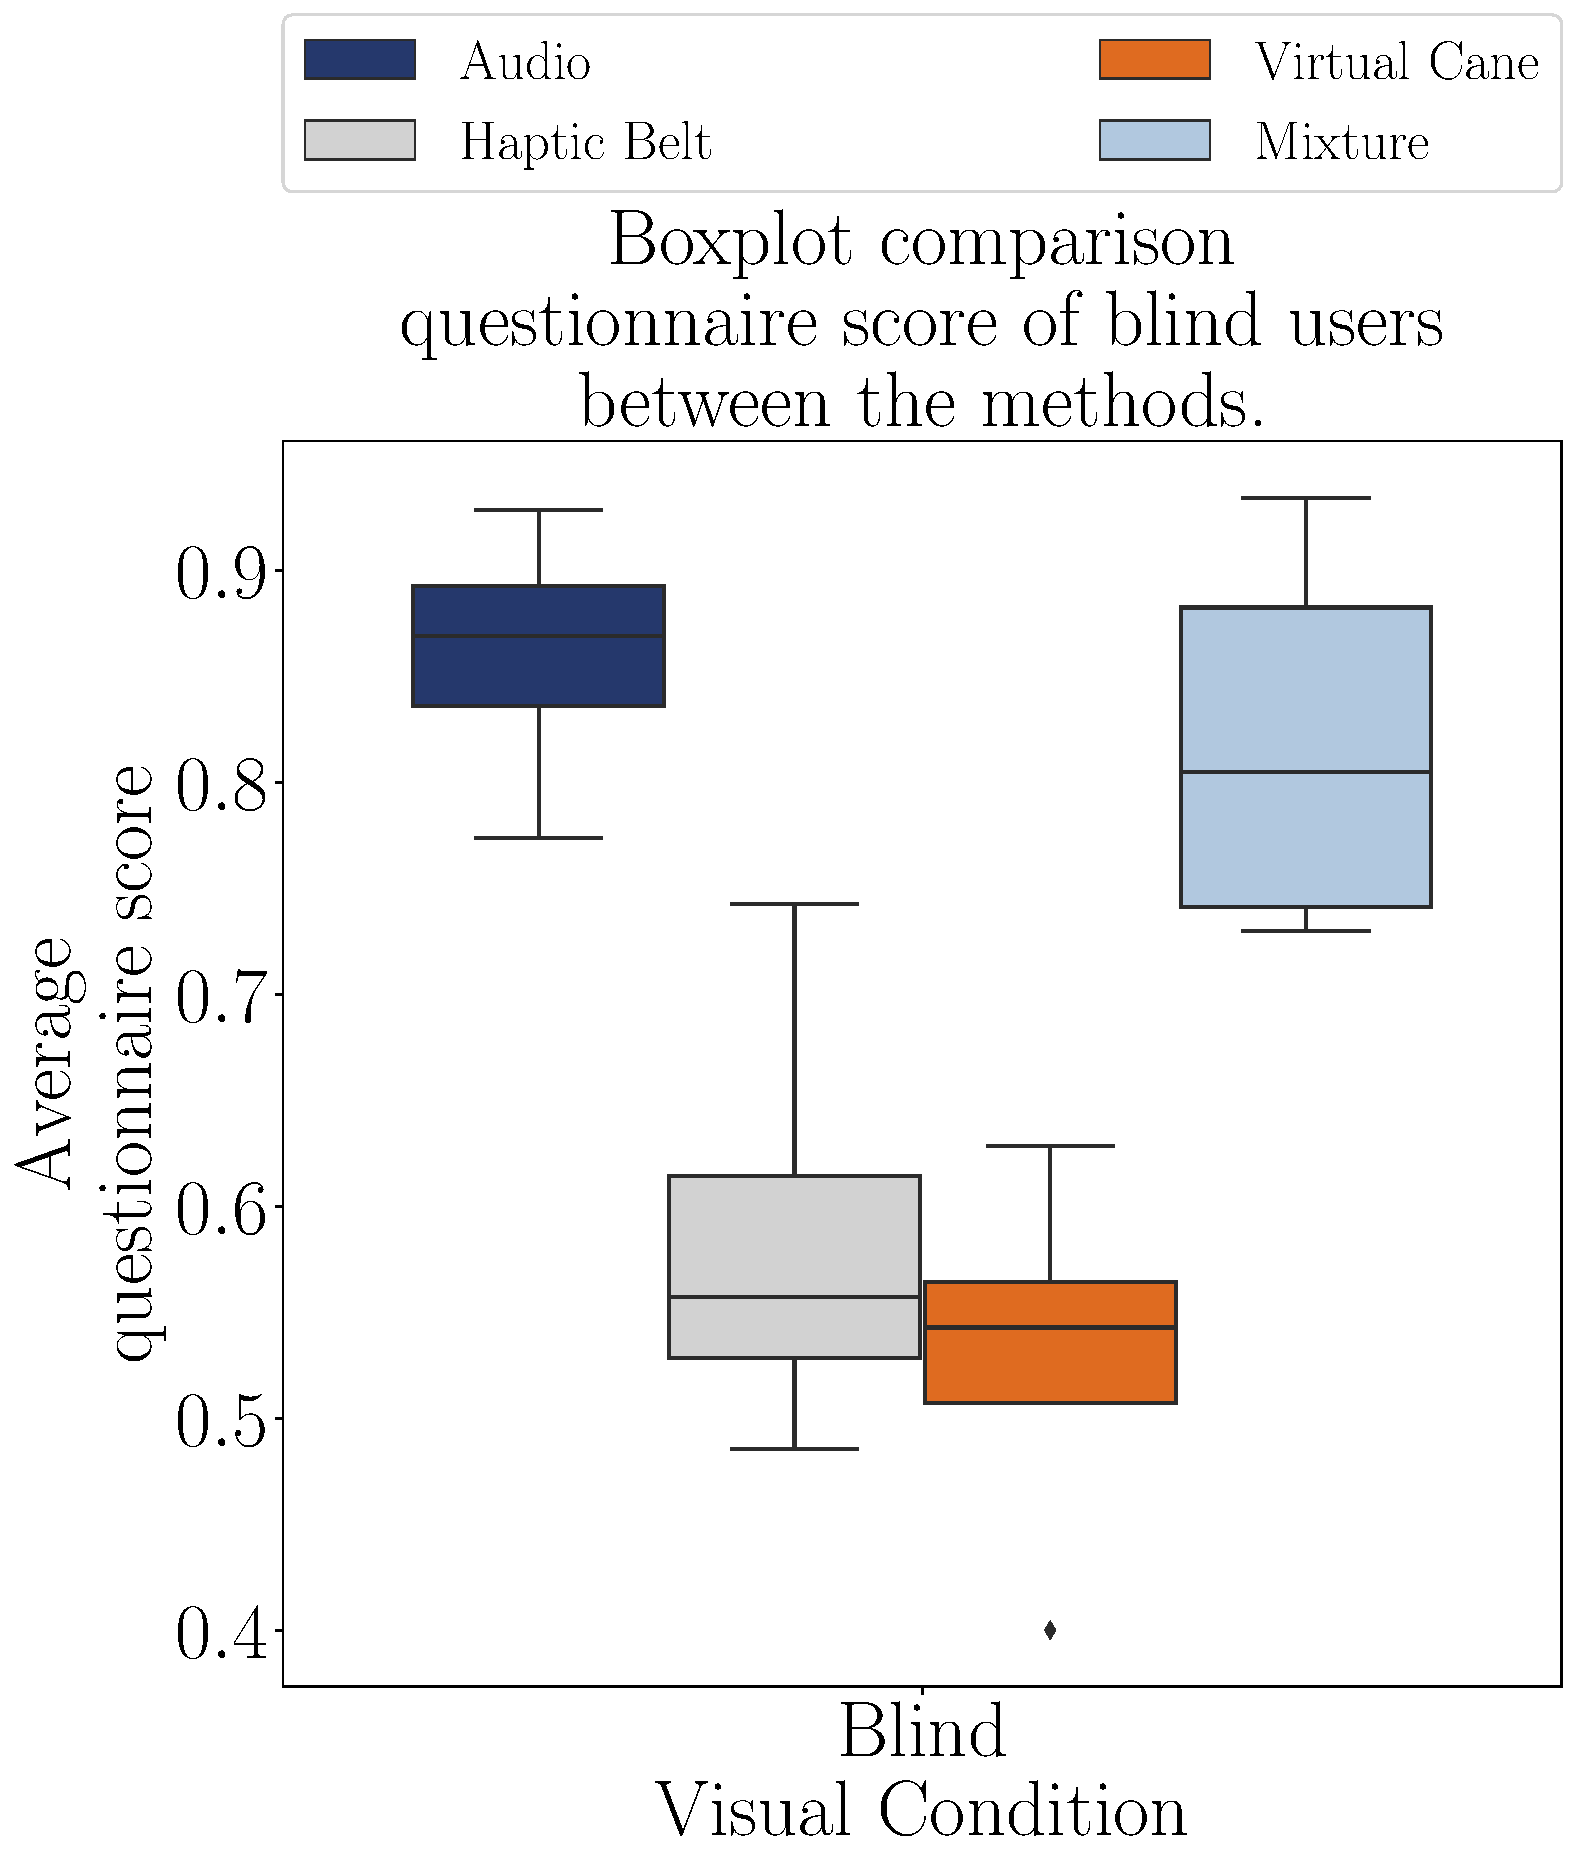
\includegraphics[width = 0.45\textwidth]{Resultados/Questionario/Figuras/pdf/boxplot_questionnaire_scene_blind.pdf}
    \caption{Boxplot of the questionaire score of the blind participants grouped by the methods.}
    \label{fig:boxplot_quest_blind_scene}
\end{figure}

%The Table \ref{tab:questionnaire_average_group_blind} show the the average questionnaire score on each method. It also shows a disatisfaction with the haptic devices alone.
%
%
\begin{table}[!htb]
\centering
\caption{Guidance method questionnaire average score for the blind participants.}
\label{tab:questionnaire_average_group_blind}
\begin{tabular}{lrrrrr}
\toprule
{} & Audio & Haptic Belt & Virtual Cane & Mixture \\
Visual Condition &       &             &              &         \\
\midrule
Blind            &  0.86 &        0.59 &         0.53 &    0.82 \\
\bottomrule
\end{tabular}
\end{table}



Figures \ref{fig:qqplot_questionnaire_blind} and \ref{fig:residplot_questionnaire_blind} show that the data follows a normal distribution. However, the residual variance is not strictly homogenous among the participants. 

\begin{figure}[!thb]
    \centering
    \begin{minipage}{0.45\textwidth}
        \centering
        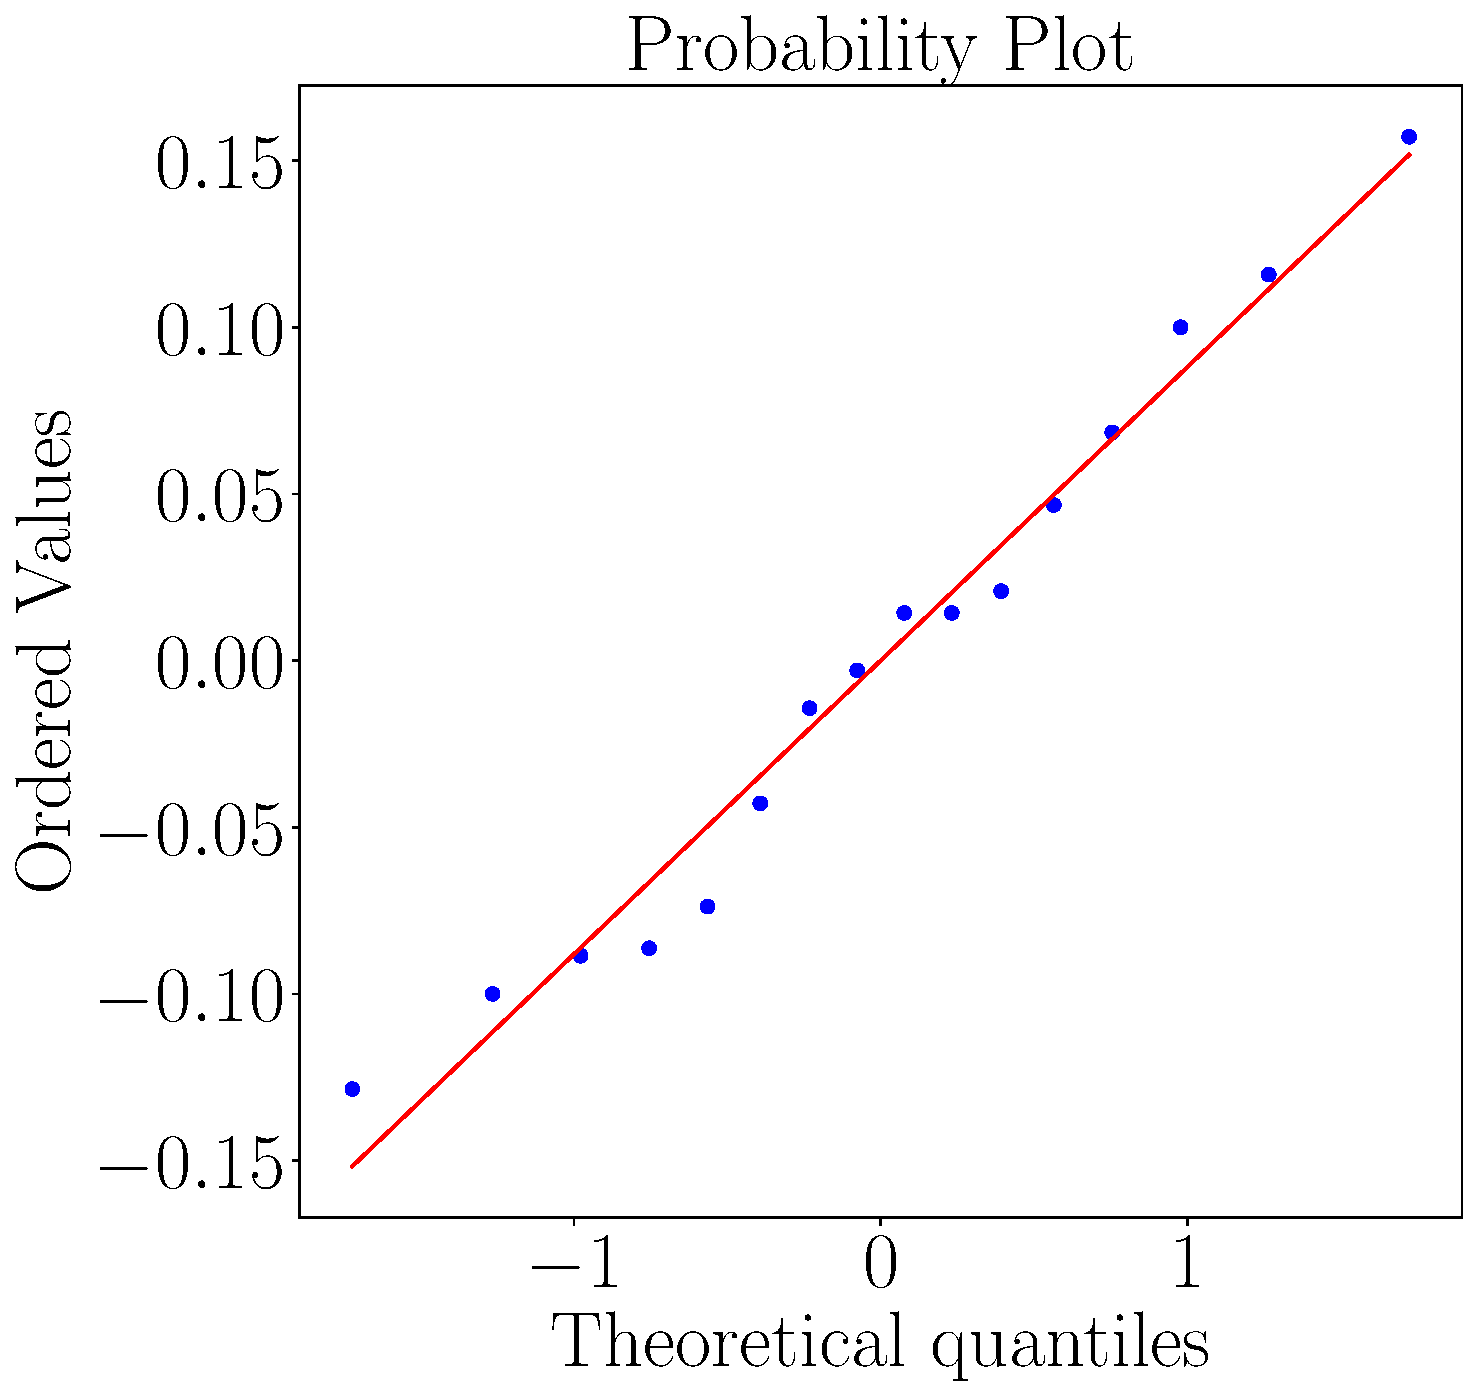
\includegraphics[width = \textwidth]{Resultados/Questionario/Figuras/pdf/qqplot_questionnaire_blind.pdf}
        \caption{QQ plot of the questionnaire score of the blind participants on each method.}
        \label{fig:qqplot_questionnaire_blind}
    \end{minipage}
    \begin{minipage}{0.075\textwidth}
        \hfill
    \end{minipage}
    \begin{minipage}{0.45\textwidth}
        \centering
        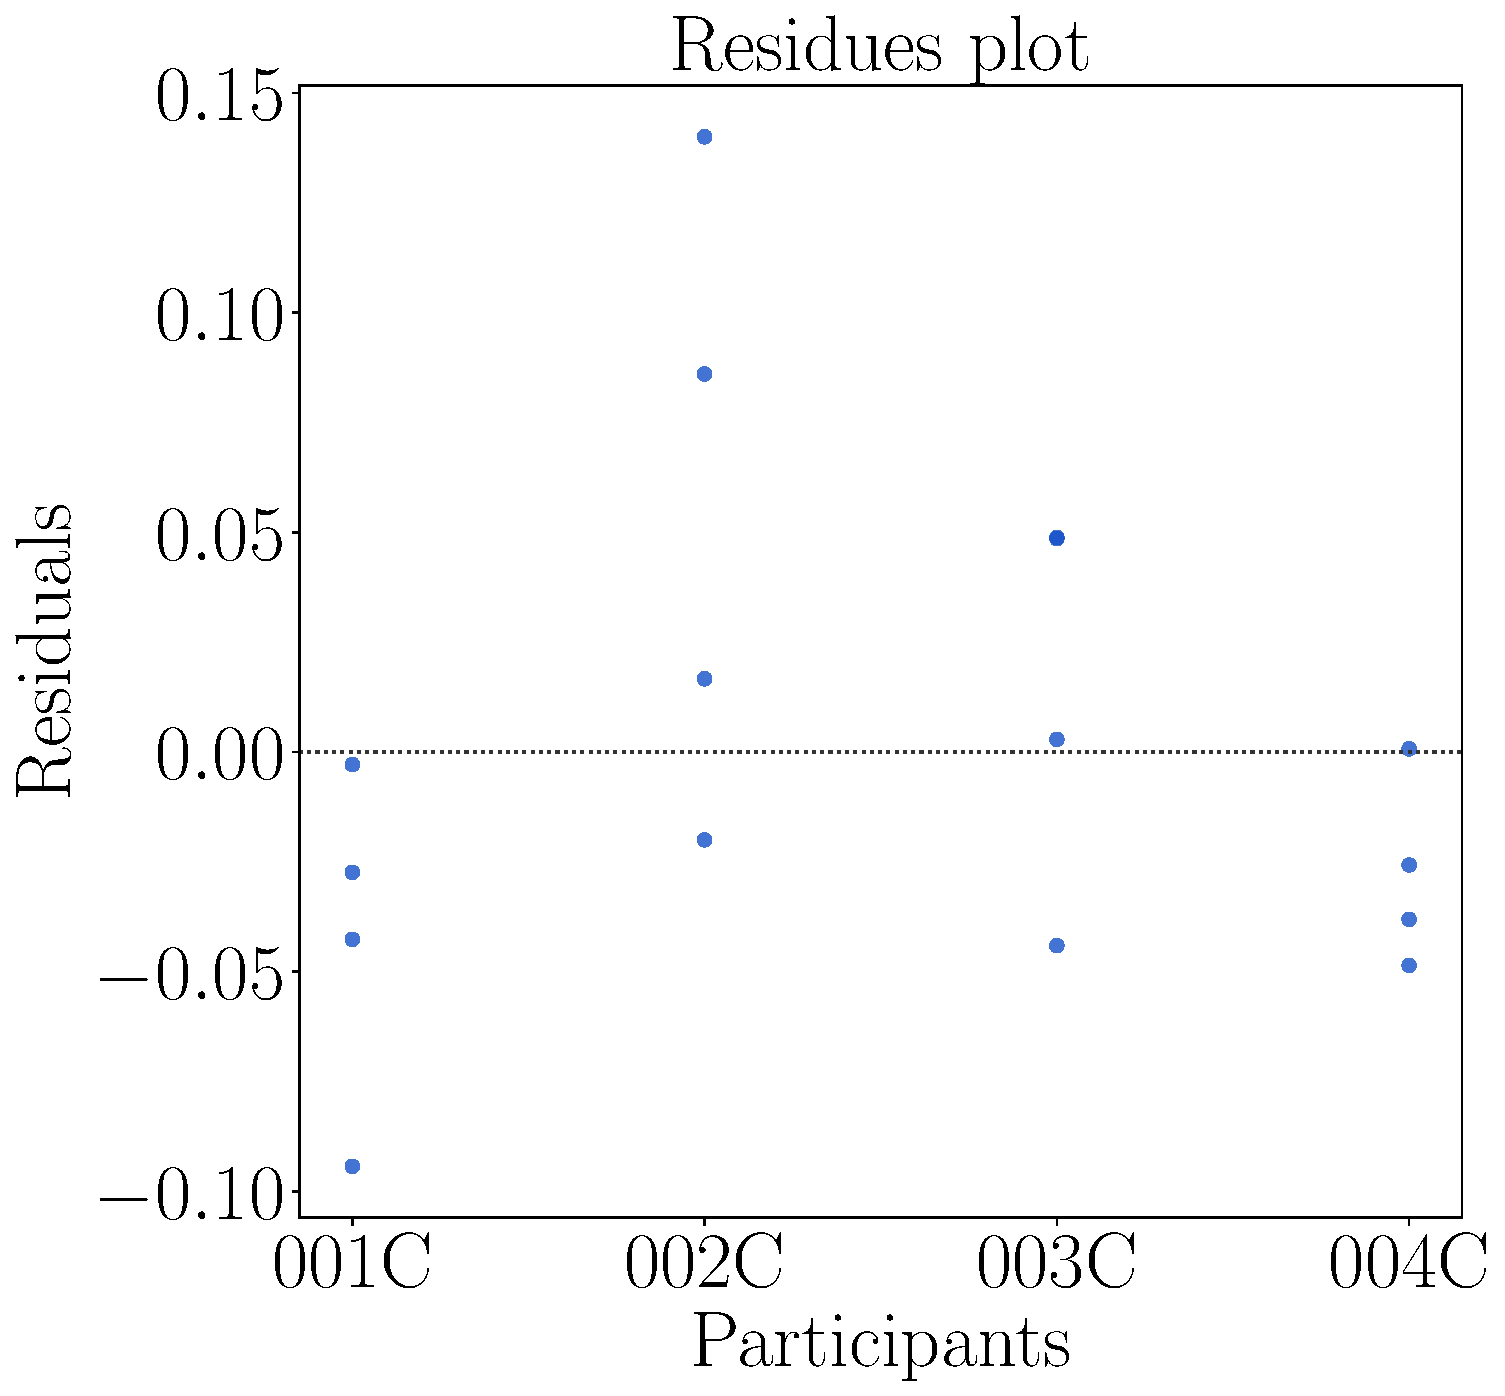
\includegraphics[width = \textwidth]{Resultados/Questionario/Figuras/pdf/residplot_questionnaire_blind.pdf}
        \caption{Residual plot of the questionnaire score the blind participants on each method.}
        \label{fig:residplot_questionnaire_blind}
    \end{minipage}
\end{figure}

The results of ANOVA are presented in Table  \ref{tab:blocanova_questionnaire_blind} and it shows that the method, with a p-value of 0.001, is indeed a significant variable that affects the user's satisfaction.


\begin{table}[!htb]
\centering
\caption{Anova p-value for the questionnaire score on each method for blinded users.}
\label{tab:blocanova_questionnaire_blind}
\begin{tabular}{lrrrrr}
\toprule
Source & P-Value \\
\midrule
Method & 0.001** \\
\bottomrule
\end{tabular}
\end{table}



In order to complement the ANOVA analysis, the pairwise comparison of the methods obtained from the Fisher LSD test is presented in Table \ref{tab:lsd_questionnaire_blind}. The results show that audio and mixture are equivalent from the perspective of user satisfaction. All the other comparisons indicate there is a difference between the methods.


\begin{table}[!htb]
\centering
\caption{Cross validation p-value for the questionnaire score on each method for blinded users.}
\label{tab:lsd_questionnaire_blind}
\begin{tabular}{rcllr}
\toprule
      \multicolumn{3}{c}{Method} &                          \multicolumn{2}{c}{Analysis} \\
\midrule
       Audio & $X$ & Haptic Belt &        $H_1 : \mu_{Audio} \ne \mu_{Haptic Belt}$ & ** \\
      Audio & $X$ & Virtual Cane &       $H_1 : \mu_{Audio} \ne \mu_{Virtual Cane}$ & ** \\
           Audio & $X$ & Mixture &                $H_0 : \mu_{Audio} = \mu_{Mixture}$ &  \\
Haptic Belt & $X$ & Virtual Cane & $H_1 : \mu_{Haptic Belt} \ne \mu_{Virtual Cane}$ & ** \\
     Haptic Belt & $X$ & Mixture &      $H_1 : \mu_{Haptic Belt} \ne \mu_{Mixture}$ & ** \\
    Virtual Cane & $X$ & Mixture &     $H_1 : \mu_{Virtual Cane} \ne \mu_{Mixture}$ & ** \\
\bottomrule
\end{tabular}
\end{table}



Additional to the scores, the participants also expressed their dissatisfaction with the answers to the open questions of the questionnaire, where they commented that the haptic belt and the virtual cane are confusing, are not precise enough, and are very different from what they are used to.

\FloatBarrier